\documentclass[a4paper,11pt]{article}
\usepackage[spanish]{babel}
\usepackage[utf8]{inputenc}
\usepackage[T1]{fontenc}
\usepackage{booktabs}
\usepackage{graphicx}
\usepackage{geometry}
\usepackage{float}
\usepackage{caption}
\usepackage{subcaption}
\usepackage{amsmath}
\usepackage{amssymb}
\usepackage{hyperref}
\usepackage{parskip}
\usepackage{xcolor}
\usepackage{array}

\geometry{margin=2.5cm}

\newcommand{\yes}{\textcolor{green!60!black}{$\checkmark$}}
\newcommand{\no}{\textcolor{red}{$\times$}}
\newcommand{\meh}{\textcolor{orange}{$\sim$}}

\title{\textbf{Resultados sobre datasets: selección de features en escenarios PU}}
\author{Verónica Vila Vivero}
\date{Marzo 2026}

\begin{document}

\maketitle
\tableofcontents
\newpage

% ===================== INTRO =====================
\section{Contexto}

El pipeline evaluado es:
\begin{enumerate}
    \item Entrenar un clasificador $P \text{ vs } U$ (regresión logística) para estimar $P(S=1 \mid x)$.
    \item Estimar $\hat{\alpha}$ a partir de esos scores.
    \item Corregir las probabilidades para obtener $\hat{P}(Y=1 \mid x)$ y calcular la MI corregida (\textbf{MI-PU}).
    \item Comparar el ranking resultante con el ranking ``naive'' (MI calculada directamente sobre $S$ en vez de $Y$) y con el ranking real (calculado con las etiquetas $Y$ verdaderas).
\end{enumerate}

La calidad del ranking se mide con la \textbf{correlación de Spearman} entre el ranking estimado y el real. Se varía $\alpha \in \{0.05, 0.1, 0.2, 0.3, 0.5\}$ con 5 semillas diferentes.

\medskip
Los resultados esperados que se quieren validar son:
\begin{enumerate}
    \item[\textbf{H1}] \textbf{MI naive falla}: confundir positivos ocultos con negativos degrada el ranking.
    \item[\textbf{H2}] \textbf{PU mejora}: la corrección propuesta debe aproximarse mejor al ranking real.
    \item[\textbf{H3}] \textbf{$\hat{\alpha}$ converge}: la estimación de $\alpha$ debe acercarse al valor verdadero.
\end{enumerate}

% ===================== BREAST CANCER =====================
\section{Breast Cancer}

\subsection{Características del dataset}

Dataset para diagnóstico de tumores de mama (\textit{Wisconsin Breast Cancer}). Contiene \textbf{569 muestras} con \textbf{30 features}. La clase positiva (tumores malignos) representa el $\approx 37\%$ de las muestras. Es un dataset limpio, bien balanceado y con features altamente informativas.

Se probaron ambas variantes con y sin ruido. \textbf{Sin ruido} sirve como \textit{baseline} controlado para verificar el comportamiento esperado. \textbf{Con ruido} simula un escenario más realista donde la calidad de las medidas clínicas puede estar degradada, algo habitual cuando las imágenes tienen artefactos o el proceso de extracción de features no es perfecto.

\subsection{Estimación de $\alpha$}

\begin{table}[H]
\centering
\caption{Estimación de $\hat{\alpha}$ -- Breast Cancer (sin ruido)}
\begin{tabular}{ccc}
\toprule
$\alpha$ real & $\hat{\alpha}$ (media) & $\hat{\alpha}$ (std) \\
\midrule
0.05 & 0.086 & 0.019 \\
0.10 & 0.161 & 0.020 \\
0.20 & 0.213 & 0.009 \\
0.30 & 0.315 & 0.014 \\
0.50 & 0.493 & 0.009 \\
\bottomrule
\end{tabular}
\end{table}

\begin{table}[H]
\centering
\caption{Estimación de $\hat{\alpha}$ -- Breast Cancer (con ruido)}
\begin{tabular}{ccc}
\toprule
$\alpha$ real & $\hat{\alpha}$ (media) & $\hat{\alpha}$ (std) \\
\midrule
0.05 & 0.124 & 0.029 \\
0.10 & 0.172 & 0.029 \\
0.20 & 0.227 & 0.004 \\
0.30 & 0.305 & 0.012 \\
0.50 & 0.478 & 0.012 \\
\bottomrule
\end{tabular}
\end{table}

\subsection{Correlación de Spearman con ranking real}

\begin{figure}[H]
\centering
\begin{subfigure}{0.48\textwidth}
    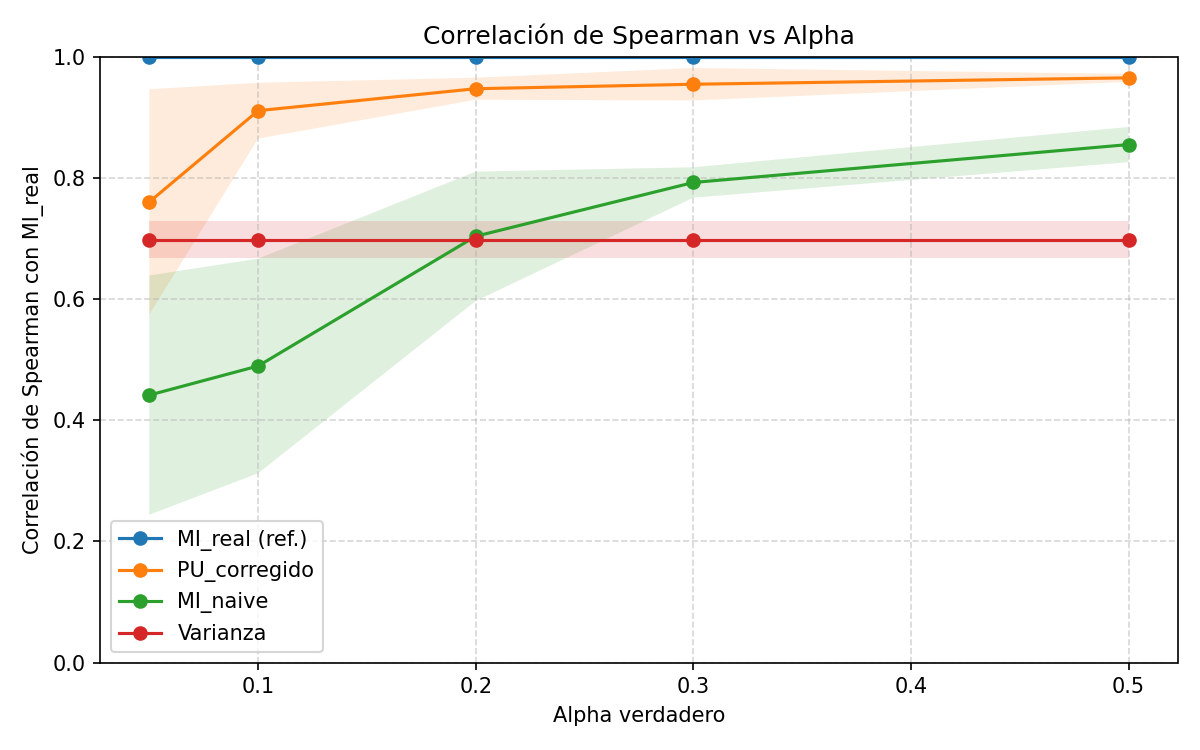
\includegraphics[width=\linewidth]{resultados/bc_spearman_vs_alpha.png}
    \caption{Sin ruido}
\end{subfigure}
\hfill
\begin{subfigure}{0.48\textwidth}
    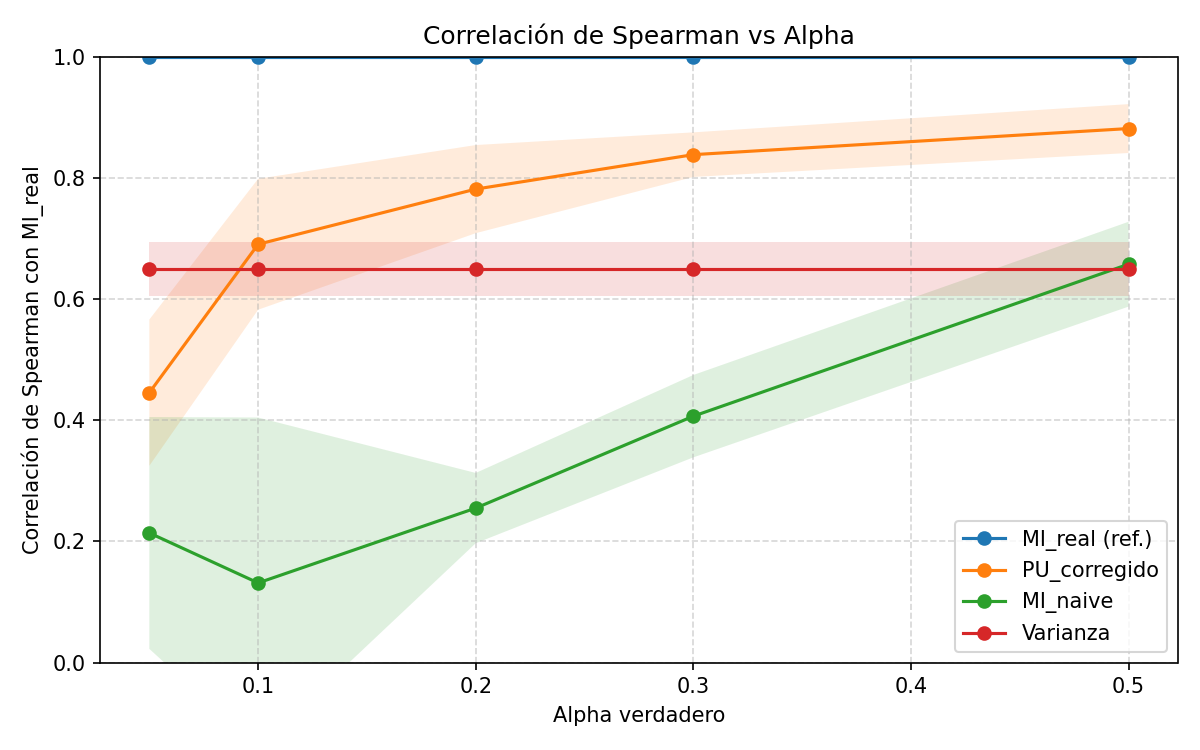
\includegraphics[width=\linewidth]{resultados/bc_ruido_spearman_vs_alpha.png}
    \caption{Con ruido}
\end{subfigure}
\caption{Breast Cancer: correlación de Spearman con el ranking real vs $\alpha$ verdadero.}
\end{figure}

\subsection{Análisis}

\textbf{Sin ruido} -- las tres hipótesis de resultados esperados se cumplen:
\begin{itemize}
    \item \textbf{H1}: el naive falla, especialmente a $\alpha$ bajos. Para $\alpha = 0.05$ la correlación naive es apenas $0.44$, confirmando que con pocos positivos etiquetados el ranking naive es pobre.
    \item \textbf{H2}: el método PU mejora claramente ($0.76$ para $\alpha=0.05$, subiendo hasta $0.97$ para $\alpha=0.5$). La diferencia con el naive es muy grande con valores bajos de $\alpha$, que es exactamente el caso esperado.
    \item \textbf{H3}: la estimación es muy cercana al valor real ($0.493$ vs $0.5$ para $\alpha=0.5$). Para $\alpha=0.05$ hay una sobreestimación de $\approx 0.04$, hay muy pocos positivos etiquetados y el clasificador tiene dificultad para calibrar los scores.
\end{itemize}

\textbf{Con ruido} -- la tendencia se mantiene pero con valores absolutos más bajos:
\begin{itemize}
    \item El ruido aumenta las estimaciones de $\hat{\alpha}$ para valores pequeños (estima $0.12$ cuando el real es $0.05$), lo que significa que la señal PU se confunde con el ruido.
    \item La correlación naive baja aún más ($0.21$ para $\alpha=0.05$), mientras que PU se mantiene por encima de $0.44$.
    \item El método PU sigue siendo claramente superior al naive. La robustez al ruido es razonable.
\end{itemize}

Breast Cancer es el dataset donde el método funciona de forma más limpia y donde se validan las tres hipótesis esperadas.

% ===================== SONAR =====================
\section{Sonar}

\subsection{Características del dataset}

Señales sonar para distinguir rocas de minas submarinas (\textit{Sonar, Mines vs Rocks}). Son \textbf{208 muestras} con \textbf{60 features} (energías de la señal en diferentes bandas de frecuencia). Es un dataset binario perfectamente balanceado ($50\%$ / $50\%$), pero difícil por la alta relación features/muestras ($60/208 \approx 0.29$).

Con tan pocas muestras, añadir ruido gaussiano extra haría los estimadores de MI demasiado complejos. Ya en bruto los resultados son muy ruidosos; el experimento con ruido no aportaría información útil y dificultaría la interpretación.

\subsection{Estimación de $\alpha$}

\begin{table}[H]
\centering
\caption{Estimación de $\hat{\alpha}$ -- Sonar}
\begin{tabular}{ccc}
\toprule
$\alpha$ real & $\hat{\alpha}$ (media) & $\hat{\alpha}$ (std) \\
\midrule
0.05 & 0.528 & 0.086 \\
0.10 & 0.442 & 0.059 \\
0.20 & 0.396 & 0.041 \\
0.30 & 0.489 & 0.042 \\
0.50 & 0.554 & 0.044 \\
\bottomrule
\end{tabular}
\end{table}

\subsection{Correlación de Spearman con ranking real}

\begin{figure}[H]
\centering
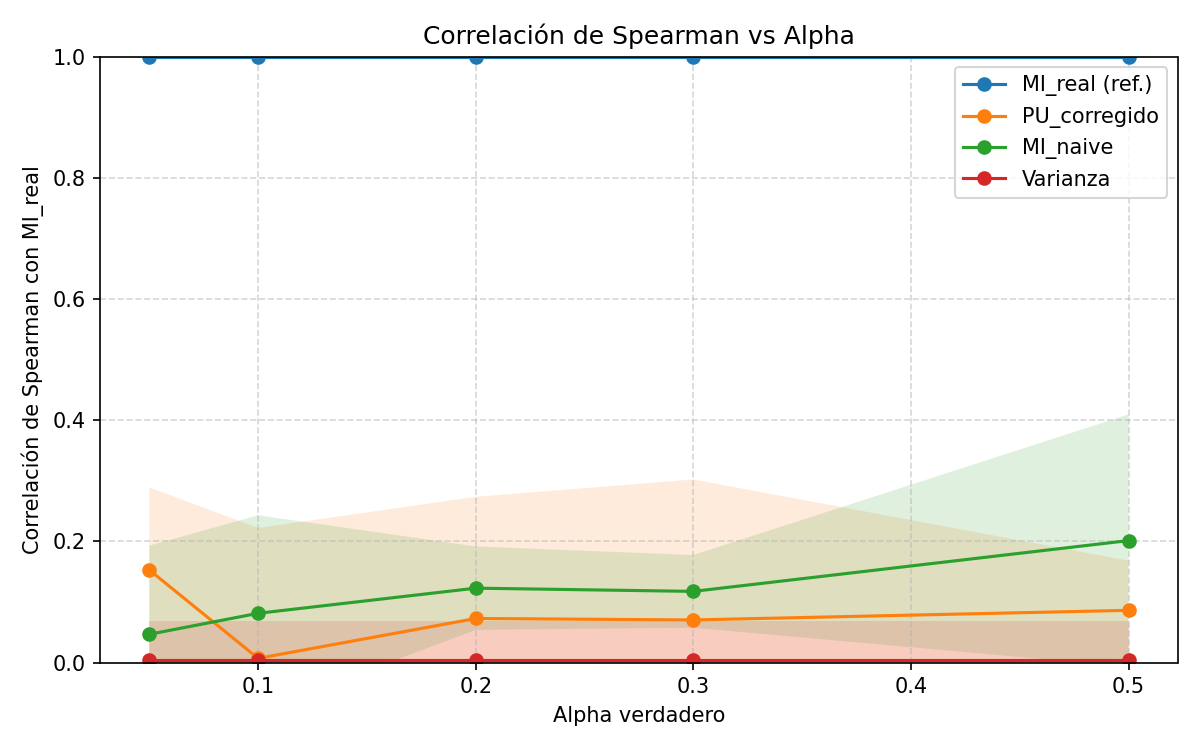
\includegraphics[width=0.65\textwidth]{resultados/sonar_spearman_vs_alpha.png}
\caption{Sonar: correlación de Spearman con el ranking real vs $\alpha$ verdadero.}
\end{figure}

\subsection{Análisis}

\begin{itemize}
    \item \textbf{H1}: el naive sí falla ($0.05$--$0.20$). El ranking naive no contiene información útil sobre el ranking real.
    \item \textbf{H2}: el PU tampoco funciona ($0.007$--$0.15$). La corrección PU no logra mejorar el ranking, sino que en algún caso lo empeora. No tiene sentido corregir con un $\hat{\alpha}$ erroneo.
    \item \textbf{H3}: la estimación de $\hat{\alpha}$ falla completamente. Independientemente del valor real, el estimador devuelve valores en torno a $0.40$--$0.55$, que corresponde aproximadamente a la proporción de positivos en el dataset ($50\%$). El clasificador logístico está sobreajustando: con $\approx 3.5$ muestras por feature, no puede aprender, y los scores $P(S=1 \mid x)$ son muy aleatorios.
\end{itemize}

El fallo lo causa el ratio muestras/features. Con tan poca información, todo el pipeline se degrada. Este dataset requeriría reducción de dimensionalidad previa (p.ej.\ PCA) o un clasificador más regularizado para que el método tuviera alguna posibilidad de funcionar.

% ===================== IONOSPHERE =====================
\section{Ionosphere}

\subsection{Características del dataset}

Señales de radar del ionosfera (\textit{Johns Hopkins Ionosphere}). Contiene \textbf{351 muestras} con \textbf{34 features} (amplitudes y fases de pulsos de radar). Clasificación binaria: señal ``buena'' (estructuras detectadas en el ionosfera) vs ``mala'' (sin retorno estructurado). Es un dataset pequeño, con features correlacionadas y una clase positiva del $\approx 64\%$.

Se probó con ruido para simular degradación de la señal radar. La pequeña muestra hace que el ruido tenga un impacto notable, lo que permite estudiar cómo de frágil es el método con pocos datos.

\subsection{Estimación de $\alpha$}

\begin{table}[H]
\centering
\caption{Estimación de $\hat{\alpha}$ -- Ionosphere (sin ruido)}
\begin{tabular}{ccc}
\toprule
$\alpha$ real & $\hat{\alpha}$ (media) & $\hat{\alpha}$ (std) \\
\midrule
0.05 & 0.093 & 0.024 \\
0.10 & 0.143 & 0.045 \\
0.20 & 0.232 & 0.025 \\
0.30 & 0.309 & 0.011 \\
0.50 & 0.470 & 0.010 \\
\bottomrule
\end{tabular}
\end{table}

\begin{table}[H]
\centering
\caption{Estimación de $\hat{\alpha}$ -- Ionosphere (con ruido)}
\begin{tabular}{ccc}
\toprule
$\alpha$ real & $\hat{\alpha}$ (media) & $\hat{\alpha}$ (std) \\
\midrule
0.05 & 0.186 & 0.067 \\
0.10 & 0.155 & 0.065 \\
0.20 & 0.239 & 0.021 \\
0.30 & 0.317 & 0.020 \\
0.50 & 0.460 & 0.021 \\
\bottomrule
\end{tabular}
\end{table}

\subsection{Correlación de Spearman con ranking real}

\begin{figure}[H]
\centering
\begin{subfigure}{0.48\textwidth}
    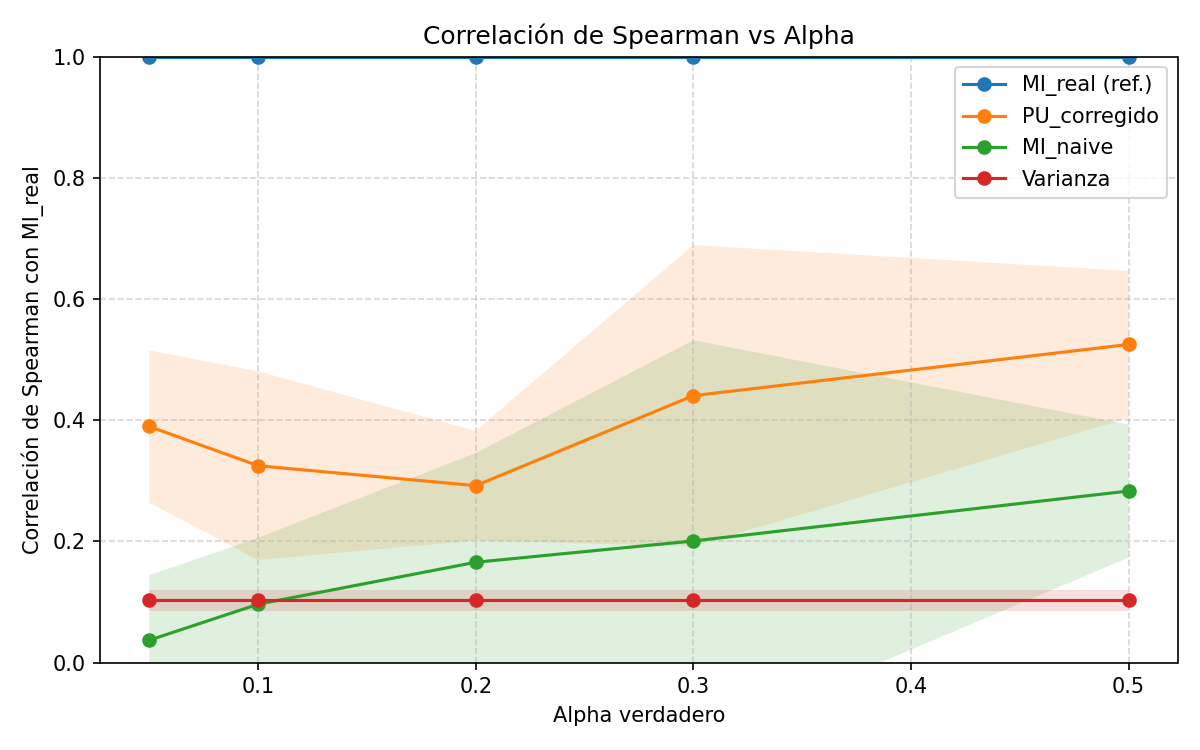
\includegraphics[width=\linewidth]{resultados/ionosphere_spearman_vs_alpha.png}
    \caption{Sin ruido}
\end{subfigure}
\hfill
\begin{subfigure}{0.48\textwidth}
    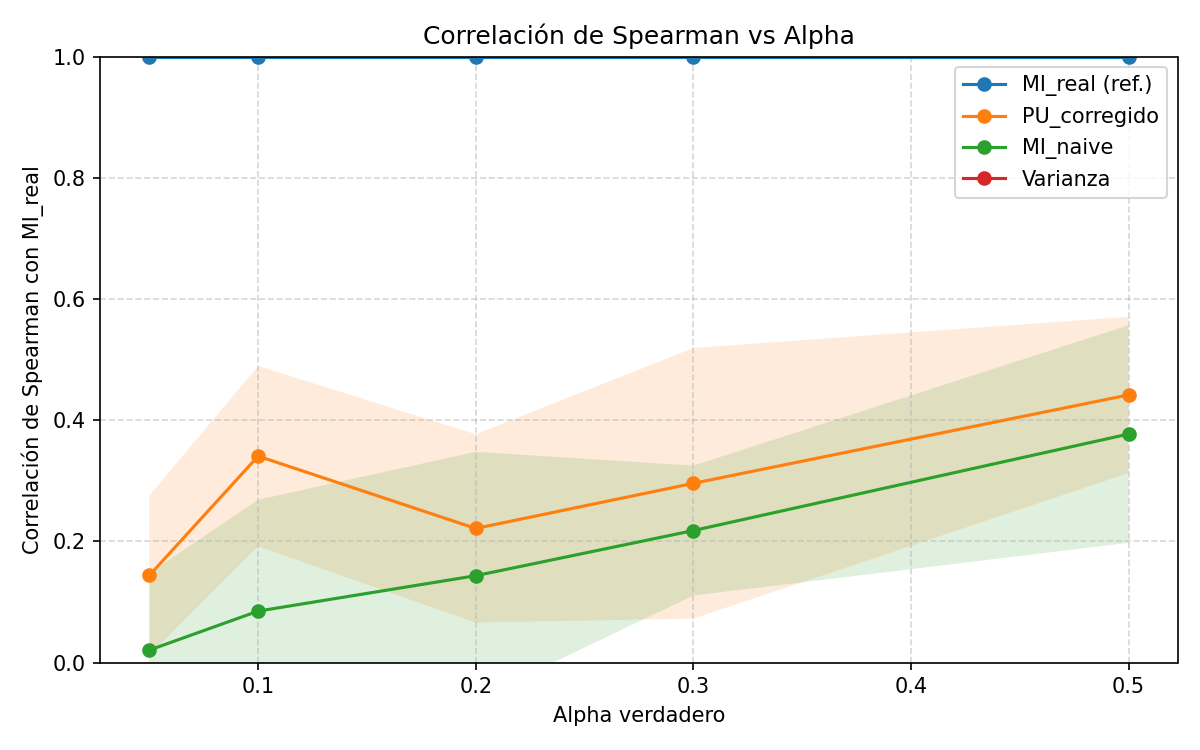
\includegraphics[width=\linewidth]{resultados/io_ruido_spearman_vs_alpha.png}
    \caption{Con ruido}
\end{subfigure}
\caption{Ionosphere: correlación de Spearman con el ranking real vs $\alpha$ verdadero.}
\end{figure}

\subsection{Análisis}

\textbf{Sin ruido:}
\begin{itemize}
    \item \textbf{H1}: el naive falla claramente. Las correlaciones naive son muy bajas ($0.04$--$0.28$), lo que confirma que las features no discriminan bien.
    \item \textbf{H2}: el PU mejora, pero poco ($0.29$--$0.53$). La mejora es real pero el resultado final no es perfecto. El tamaño del dataset (351 muestras) limita la calidad de todas las estimaciones de MI. Además, las features de radar están fuertemente correlacionadas, lo que hace inestable el ranking entre semillas.
    \item \textbf{H3}: la estimación es razonablemente buena para $\alpha \geq 0.2$. Para $\alpha = 0.05$ casi dobla el valor real ($0.093$ vs $0.05$), lo que es esperable con tan pocos positivos etiquetados en una muestra pequeña.
\end{itemize}

\textbf{Con ruido:} los resultados empeoran en todos los aspectos. Destaca que $\hat{\alpha}$ para $\alpha = 0.05$ sube hasta $0.186$, y la desviación estándar es alta ($0.067$). La correlación PU baja especialmente para $\alpha=0.05$ ($0.144$). El ruido, combinado con el pequeño tamaño de muestra, hace muy inestable el clasificador PU.

Los resultados son parcialmente satisfactorios; la limitación principal es el tamaño reducido del dataset, que impide que las estimaciones de MI tengan suficiente potencia estadística.

% ===================== GAS SENSOR =====================
\section{Gas Sensor Drift}

\subsection{Características del dataset}

Dataset de la UCI de sensores de gas con deriva temporal (\textit{Gas Sensor Array Drift}). Contiene \textbf{13{,}910 muestras} con \textbf{128 features} (respuestas de 16 sensores químicos metálicos para 6 tipos de gas). Se trabajó con una versión binaria adaptada al escenario PU. Es un dataset de alta dimensión con fuerte señal discriminativa.

Los sensores de gas sufren deriva temporal real, por lo que el experimento \textbf{con ruido} simula degradación adicional de la señal. La variante \textbf{batch} divide los datos en lotes temporales correspondientes a distintas campañas de medición, que es la estructura original del dataset.

\subsection{Estimación de $\alpha$}

\begin{table}[H]
\centering
\caption{Estimación de $\hat{\alpha}$ -- Gas Sensor (sin ruido)}
\begin{tabular}{ccc}
\toprule
$\alpha$ real & $\hat{\alpha}$ (media) & $\hat{\alpha}$ (std) \\
\midrule
0.05 & 0.058 & 0.006 \\
0.10 & 0.103 & 0.005 \\
0.20 & 0.198 & 0.005 \\
0.30 & 0.288 & 0.006 \\
0.50 & 0.474 & 0.003 \\
\bottomrule
\end{tabular}
\end{table}

\begin{table}[H]
\centering
\caption{Estimación de $\hat{\alpha}$ -- Gas Sensor (con ruido)}
\begin{tabular}{ccc}
\toprule
$\alpha$ real & $\hat{\alpha}$ (media) & $\hat{\alpha}$ (std) \\
\midrule
0.05 & 0.078 & 0.006 \\
0.10 & 0.104 & 0.006 \\
0.20 & 0.169 & 0.007 \\
0.30 & 0.243 & 0.004 \\
0.50 & 0.389 & 0.008 \\
\bottomrule
\end{tabular}
\end{table}

\begin{table}[H]
\centering
\caption{Estimación de $\hat{\alpha}$ -- Gas Sensor (batch 1)}
\begin{tabular}{ccc}
\toprule
$\alpha$ real & $\hat{\alpha}$ (media) & $\hat{\alpha}$ (std) \\
\midrule
0.05 & 0.111 & 0.046 \\
0.10 & 0.143 & 0.036 \\
0.20 & 0.223 & 0.027 \\
0.30 & 0.300 & 0.025 \\
0.50 & 0.454 & 0.014 \\
\bottomrule
\end{tabular}
\end{table}

\subsection{Correlación de Spearman con ranking real}

\begin{figure}[H]
\centering
\begin{subfigure}{0.32\textwidth}
    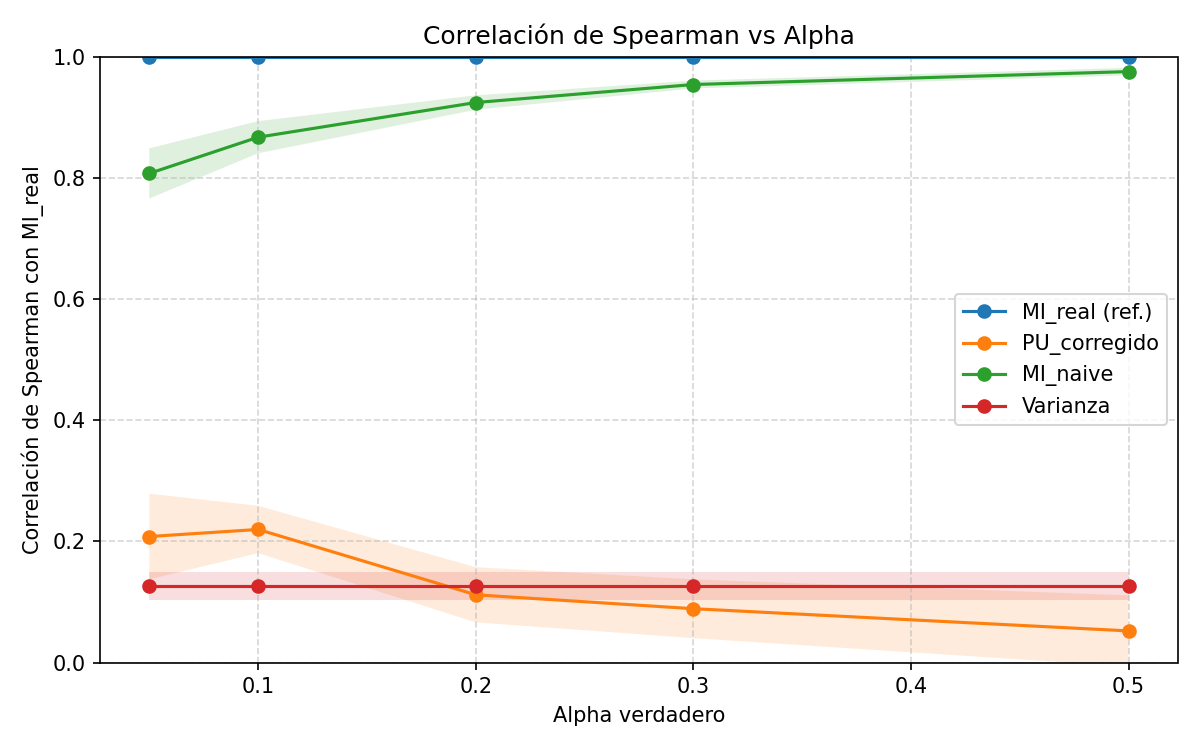
\includegraphics[width=\linewidth]{resultados/gas_spearman_vs_alpha.png}
    \caption{Sin ruido}
\end{subfigure}
\hfill
\begin{subfigure}{0.32\textwidth}
    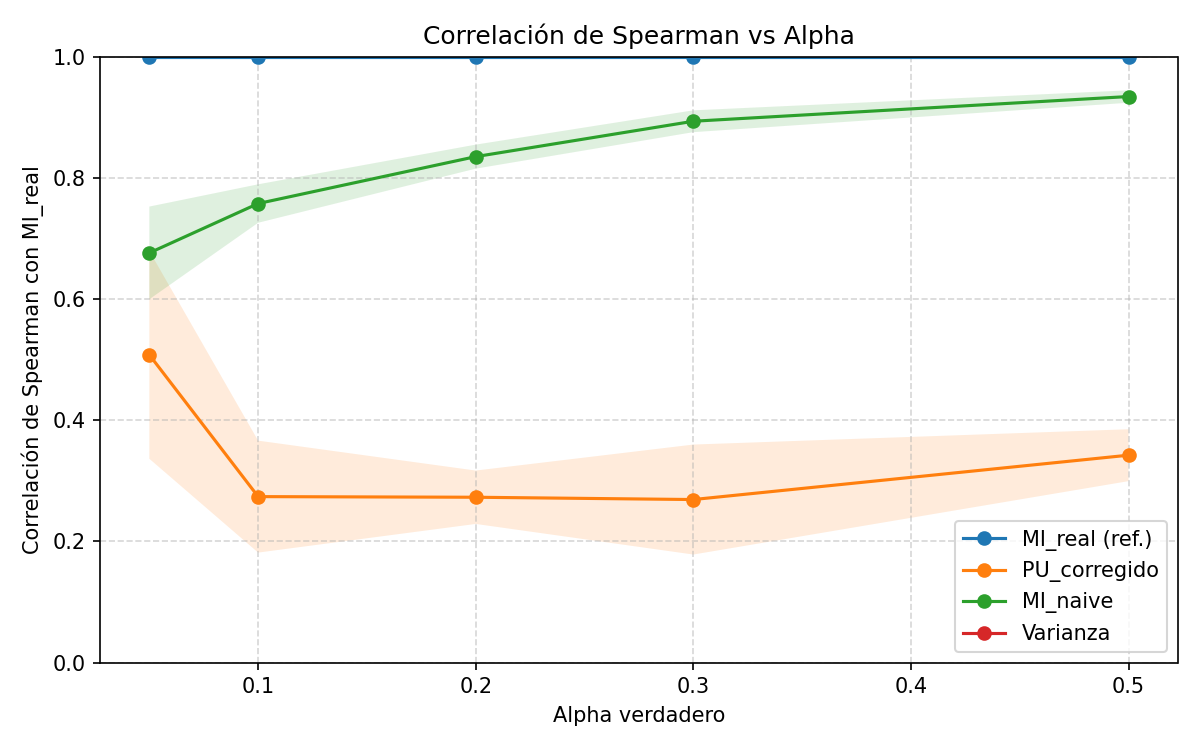
\includegraphics[width=\linewidth]{resultados/gas_ruido_spearman_vs_alpha.png}
    \caption{Con ruido}
\end{subfigure}
\hfill
\begin{subfigure}{0.32\textwidth}
    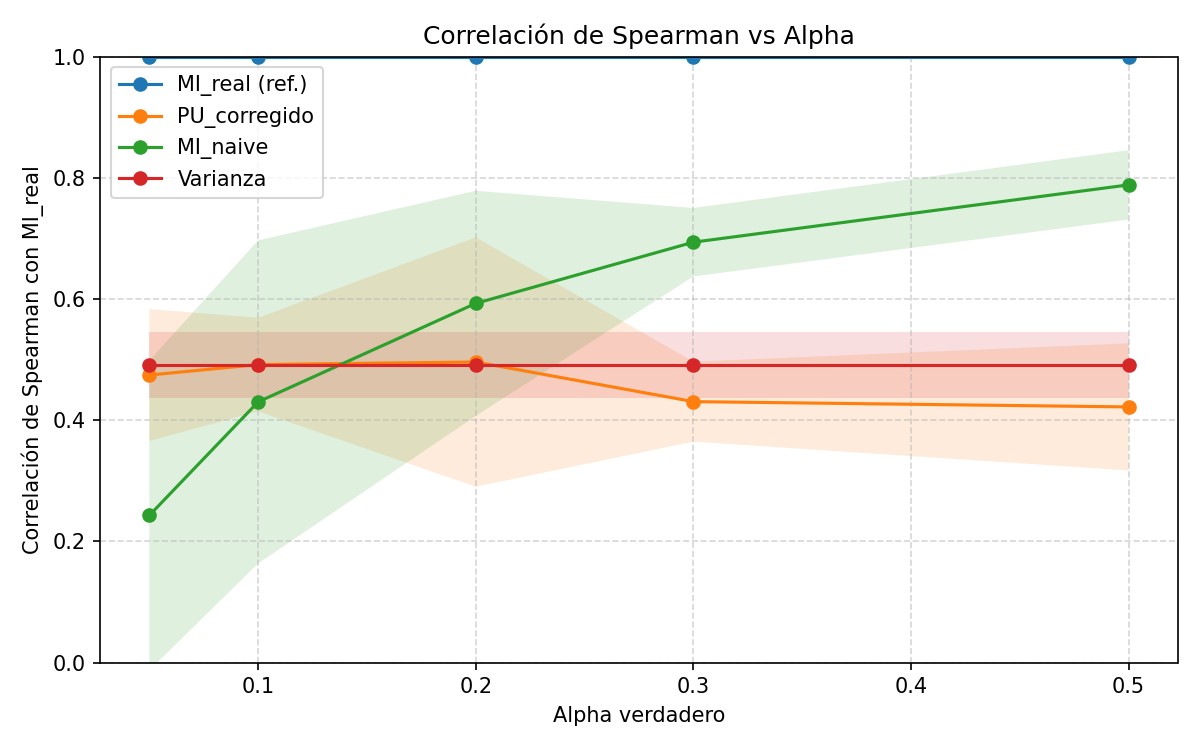
\includegraphics[width=\linewidth]{resultados/gas_batch_spearman_vs_alpha.png}
    \caption{Batch}
\end{subfigure}
\caption{Gas Sensor Drift: correlación de Spearman con el ranking real vs $\alpha$ verdadero.}
\end{figure}

\subsection{Análisis}

\textbf{Gas Sensor Drift es un dataset multiclase, no binario}, y este es el problema que explica todos los resultados anómalos que se observan.

El dataset original contiene \textbf{6 clases de gas} (Ethanol, Ethylene, Ammonia, Acetaldehyde, Acetone, Toluene). Para poder aplicar el framework PU se elige una de las 6 clases como ``positivo'' y se etiquetan todas las demás como ``negativo''. Esto genera un conjunto de negativos \textbf{heterogéneo}: no son muestras de una clase coherente, sino la unión de 5 tipos de gas completamente diferentes entre sí, cada uno con su propia distribución en el espacio de features.

Este diseño rompe un supuesto fundamental del método PU: que los negativos (unlabeled que son realmente negativos) provienen de una distribución homogénea y bien definida. En la práctica ocurre lo siguiente:

\begin{itemize}
    \item El clasificador $P$ vs $U$ no aprende a separar ``este gas'' de ``no este gas'', sino que intenta construir una frontera entre una clase compacta y una mezcla de 5 distribuciones muy distintas. Aunque la mezcla de negativos cubre regiones del espacio de features muy alejadas de los positivos, haciendo la separación $P$ vs $U$ trivialmente lineal y con altos scores incluso sin corrección PU.
    \item Como consecuencia, los scores $\hat{P}(S=1 \mid x)$ capturan principalmente ``pertenencia a la clase del positivo'' de forma casi perfecta, lo que explica que $\hat{\alpha}$ converja bien (H3). Pero esta separación: no se debe a que el método PU funcione, sino a que los negativos heterogéneos son fácilmente distinguibles en nivel de features.
    \item El ranking de features refleja qué sensores discriminan mejor entre las 6 clases de gas globalmente, no qué sensores son informativos desde la perspectiva binaria positivo/negativo. Por eso el naive, que usa directamente las etiquetas binarizadas, ya captura ese ranking correctamente sin necesitar ninguna corrección.
\end{itemize}

En un dataset verdaderamente binario, los positivos ocultos en el unlabeled se confunden con los negativos y degradan el ranking naive (H1). Aquí eso no ocurre porque la señal discriminativa de los sensores es tan fuerte y la separación entre las 6 clases tan clara que el ruido PU queda enmascarado.

\textbf{Conclusión:} los resultados de Gas Sensor no invalidan el método propuesto: el método asume negativos aproximadamente i.i.d.\ de una única distribución. Cuando los negativos son una mezcla de múltiples clases heterogéneas, el escenario PU deja de ser el que el método estudia.

% ===================== MINIBOONE =====================
\section{MiniBooNE}

\subsection{Características del dataset}

Es el dataset más grande del conjunto: \textbf{130{,}065 muestras} con \textbf{50 features} (variables cinemáticas de las partículas). La clase positiva (eventos de neutrino $\nu_e$) representa el $\approx 72\%$ de las muestras, lo que implica un fuerte desbalance hacia el positivo.

Dado el enorme número de muestras, el dataset ya tiene suficiente variabilidad estadística para todos los estimadores. Añadir ruido gaussiano artificial no aportaría información nueva sobre el comportamiento del método.

\subsection{Estimación de $\alpha$}

\begin{table}[H]
\centering
\caption{Estimación de $\hat{\alpha}$ -- MiniBooNE (comparación: media vs robusto)}
\begin{tabular}{ccccc}
\toprule
$\alpha$ real & $\hat{\alpha}$ (media) & Error (media) & $\hat{\alpha}$ (robusto) & Error (robusto) \\
\midrule
0.05 & 0.029 & 42\% & 0.145 & 190\% \\
0.10 & 0.059 & 41\% & 0.192 & 92\% \\
0.20 & 0.123 & 38\% & 0.312 & 56\% \\
0.30 & 0.188 & 37\% & 0.425 & 42\% \\
0.50 & 0.319 & 36\% & 0.638 & 28\% \\
\bottomrule
\end{tabular}
\end{table}

\subsection{Correlación de Spearman con ranking real}

\begin{figure}[H]
\centering
\begin{subfigure}{0.48\textwidth}
    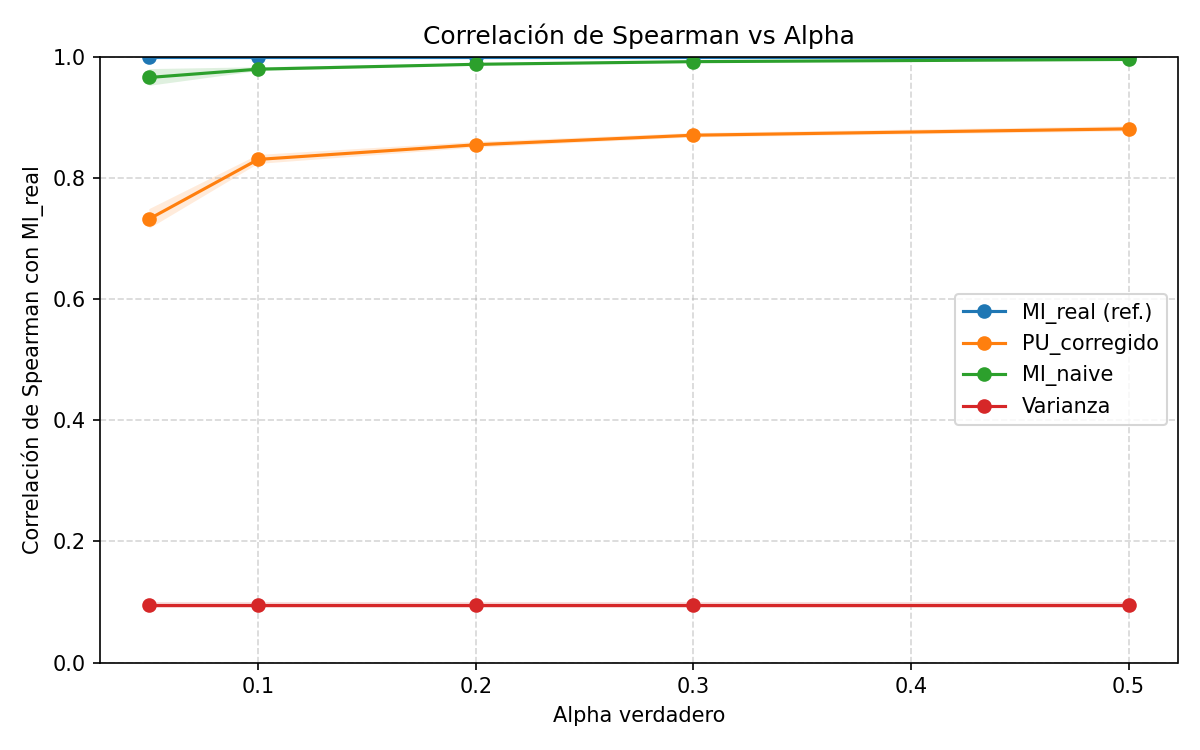
\includegraphics[width=\linewidth]{resultados/miniboone_spearman_vs_alpha.png}
    \caption{Método simple (media)}
\end{subfigure}
\hfill
\begin{subfigure}{0.48\textwidth}
    \includegraphics[width=\linewidth]{resultados/miniboone_spearman_positivos.png}
    \caption{Método robusto (positivos confiables)}
\end{subfigure}
\caption{MiniBooNE: correlación de Spearman con el ranking real vs $\alpha$ verdadero (comparación de métodos).}
\end{figure}

\subsection{Análisis}

\begin{itemize}
    \item \textbf{H1}: el naive no falla; de hecho funciona casi perfectamente ($0.97$--$1.0$). La razón es que la clase positiva es mayoritaria ($72\%$): incluso con $\alpha = 0.05$, hay tantos positivos ``ocultos'' en el unlabeled que la señal de las features relevantes no desaparece. El naive ``intuye'' el ranking correcto.
    \item \textbf{H2}: el PU también funciona bien ($0.73$--$0.88$), pero por debajo del naive. La corrección PU introduce algo de ruido en un caso donde el naive ya es casi óptimo. No hay margen de mejora porque la línea base es muy alta.
    \item \textbf{H3}: este es el fallo más significativo. La estimación de $\hat{\alpha}$ \emph{subestima sistemáticamente} el valor real. Para $\alpha = 0.5$ estima apenas $0.319$, y para $\alpha = 0.05$ estima $0.029$ cuando debería ser $0.05$. La causa probable es el fuerte desbalance de clases: como la mayoría de muestras son positivos, el conjunto unlabeled está dominado por positivos, y el clasificador PU aprende que $P(S=1 \mid x) > 0$ para casi todas las muestras, lo que colapsa el estimador de $\alpha$ hacia abajo.
\end{itemize}

MiniBooNE muesta una limitación del método porque asume una prevalencia de clases moderada. Con muchos más positivos, ni el naive falla ni $\hat{\alpha}$ converge bien.
\subsubsection{Método robusto: positivos confiables}

El método robusto de estimación de $\alpha$ (top 20\% de scores) produce un comportamiento \textbf{fuertemente dependiente de $\alpha$} en MiniBooNE:

\begin{itemize}
    \item A valores \textbf{altos de $\alpha$}: la robustez mejora significativamente. Para $\alpha=0.5$: error se reduce de 36\% a 28\%, una mejora de 8 puntos.
    \item A valores \textbf{bajos de $\alpha$}: la robustez empeora dramáticamente. Para $\alpha=0.05$: error aumenta de 42\% a 190\%, una degradación severa que refleja sobreestimación extrema.
    \item El patrón sugiere que el método robusto introduce \textbf{sesgo de sobreestimación} en MiniBooNE, especialmente problemático en el régimen de baja $\alpha$ donde los positivos etiquetados son escasos.
\end{itemize}

El ranking naive permanece robusto ($0.97$--$0.99$) y superior al PU en ambos métodos de estimación de $\alpha$. Con clase positiva mayoritaria (72\%), aunque el método robusto logra mejorar $\hat{\alpha}$ a valores altos de $\alpha$, la mejora no se traduce en mejor ranking PU. MiniBooNE demuestra que el desbalance de clases mayoría mayoritaria crea un escenario donde incluso estimaciones ``correctas'' de $\alpha$ no pueden mejorar el PU: no es el estimador el problema fundamental, sino la asimetría de clases que hace que el naive sea ya óptimo.
% ===================== SPAMBASE =====================
\section{Spambase}

\subsection{Características del dataset}

Dataset de detección de spam (\textit{Spambase}). Contiene \textbf{4{,}601 muestras} con \textbf{57 features} (frecuencias relativas de palabras y caracteres clave, además de estadísticas de longitud de palabras en mayúsculas). La clase positiva (correos spam) representa el $\approx 39\%$.

Las features de Spambase son estadísticas de texto ya procesadas (frecuencias de palabras normalizadas), no señales físicas. Añadir ruido gaussiano sobre frecuencias no tiene una interpretación semántica clara. Además, con más de 4{,}000 muestras las estimaciones son estables sin necesidad de perturbaciones adicionales.

\subsection{Estimación de $\alpha$}

\begin{table}[H]
\centering
\caption{Estimación de $\hat{\alpha}$ -- Spambase (comparación: media vs robusto)}
\begin{tabular}{ccccc}
\toprule
$\alpha$ real & $\hat{\alpha}$ (media) & Error (media) & $\hat{\alpha}$ (robusto) & Error (robusto) \\
\midrule
0.05 & 0.055 & 10\% & 0.061 & 22\% \\
0.10 & 0.090 & 10\% & 0.122 & 22\% \\
0.20 & 0.166 & 17\% & 0.240 & 20\% \\
0.30 & 0.246 & 18\% & 0.358 & 19\% \\
0.50 & 0.399 & 20\% & 0.581 & 16\% \\
\bottomrule
\end{tabular}
\end{table}

\subsection{Correlación de Spearman con ranking real}

\begin{figure}[H]
\centering
\begin{subfigure}{0.48\textwidth}
    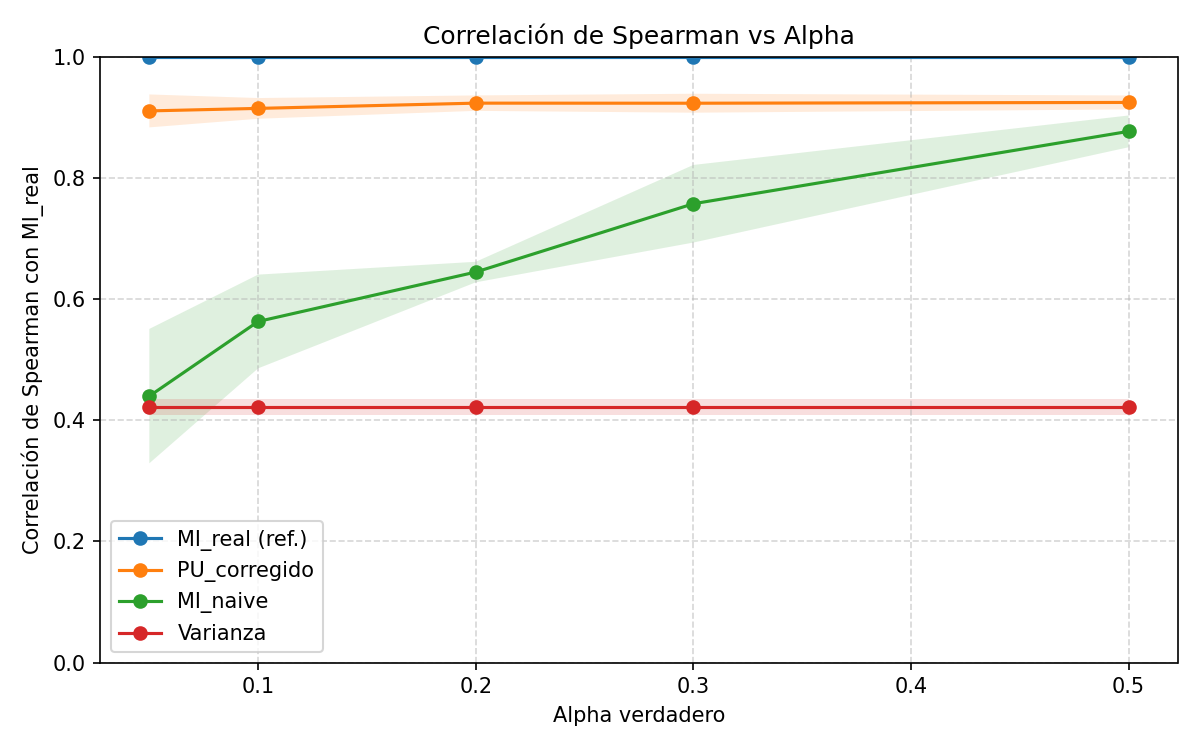
\includegraphics[width=\linewidth]{resultados/spambase_spearman_vs_alpha.png}
    \caption{Método simple (media)}
\end{subfigure}
\hfill
\begin{subfigure}{0.48\textwidth}
    \includegraphics[width=\linewidth]{resultados/spambase_spearman_positivos.png}
    \caption{Método robusto (positivos confiables)}
\end{subfigure}
\caption{Spambase: correlación de Spearman con el ranking real vs $\alpha$ verdadero (comparación de métodos).}
\end{figure}

\subsection{Análisis}

\begin{itemize}
    \item \textbf{H1}: el naive falla a $\alpha$ bajos ($0.44$ para $\alpha=0.05$) y mejora con $\alpha$ ($0.88$ para $\alpha=0.5$), confirmando la hipótesis de degradación.
    \item \textbf{H2}: el PU obtiene $0.91$--$0.92$ \emph{independientemente de $\alpha$}. El método PU aísla correctamente las features informativas sobre el spam sin que el nivel de etiquetado parcial le afecte. Para $\alpha=0.05$, el naive da $0.44$ mientras el PU da $0.91$: una diferencia de casi $0.5$ puntos de correlación.
    \item \textbf{H3}: la estimación converge bien para $\alpha$ pequeños pero subestima para $\alpha=0.5$ ($0.399$ vs $0.5$). El error es pequeño y no parece afectar a la calidad del ranking PU.
\end{itemize}

Spambase presenta un comportamiento razonablemente bueno, pero con limitaciones. Aunque el Spearman PU se mantiene en $0.91$--$0.92$ independientemente de $\alpha$ (mejora consistente sobre el naive), estos valores no alcanzan excelencia: a $\alpha$ bajo ($0.05$) el naive con $0.44$ todavía deja margen de error notable incluso en el mejor caso PU. La falta de variabilidad con $\alpha$ es deseable en la práctica, pero no compensa la estabilidad de los features: la invariabilidad sugiere que el método PU logra capturar un ranking consistente, aunque no necesariamente muy diferente del que podría obtenerse con métodos más simples una vez $\alpha$ es conocido con precisión razonable.

\subsubsection{Método robusto: positivos confiables}

Se evaluó la estimación robusta de $\alpha$ (top 20\%) en Spambase. Los resultados muestran mejora marginal en $\hat{\alpha}$:

\begin{itemize}
    \item Para $\alpha = 0.5$: $\hat{\alpha}_{\text{media}} = 0.399$ (error 20\%) vs $\hat{\alpha}_{\text{robusto}} = 0.581$ (error 16\%) — mejora de 4 puntos de error
    \item Para $\alpha = 0.05$: $\hat{\alpha}_{\text{media}} = 0.055$ (error 10\%) vs $\hat{\alpha}_{\text{robusto}} = 0.061$ (error 22\%) — empeora a $\alpha$ bajo
    \item Correlación Spearman PU se mantiene en $0.900$--$0.922$ en ambos métodos, sin diferencia perceptible
\end{itemize}

La evaluación crítica es que aunque la robustez mejora $\hat{\alpha}$ a $\alpha$ alto, el beneficio es modesto (4 puntos) y la mejora no se traduce en cambio observable en el ranking PU. Adicionalmente, a $\alpha$ bajo la robustez empeora significativamente ($10\% \to 22\%$ de error), sugiriendo que el método introduce artefactos cuando la información es escasa. El Spearman invariante a $\alpha$ persiste incluso bajo ambos estimadores, indicando que la estabilidad del ranking es más atribuible a la estructura del dataset que al refinamiento de $\hat{\alpha}$.

% ===================== MAGIC TELESCOPE =====================
\section{MAGIC Telescope}

\subsection{Características del dataset}

Dataset de observación astronómica del telescopio MAGIC. Contiene \textbf{19\,020 muestras} con \textbf{10 features}. La clase positiva representa aproximadamente el \textbf{35\%} del dataset, siendo un balance muy controlado e ideal para el análisis PU.

No se aplicó ruido gaussiano adicional porque los valores de features ya representan una señal procesada. El ruido en observaciones astronómicas está intrínseco en los datos.

\subsection{Estimación de $\alpha$}

\begin{table}[H]
\centering
\caption{Estimación de $\hat{\alpha}$ -- MAGIC Gamma Telescope (comparación: media vs robusto)}
\begin{tabular}{ccccc}
\toprule
$\alpha$ real & $\hat{\alpha}$ (media) & Error (media) & $\hat{\alpha}$ (robusto) & Error (robusto) \\
\midrule
0.05 & 0.0391 & 22\% & 0.0547 & 9\% \\
0.10 & 0.0770 & 23\% & 0.1056 & 6\% \\
0.20 & 0.1540 & 23\% & 0.2077 & 4\% \\
0.30 & 0.2314 & 23\% & 0.3108 & 4\% \\
0.50 & 0.3868 & 23\% & 0.5095 & 2\% \\
\bottomrule
\end{tabular}
\end{table}

\subsection{Correlación de Spearman con ranking real}

\begin{figure}[H]
\centering
\begin{subfigure}{0.48\textwidth}
    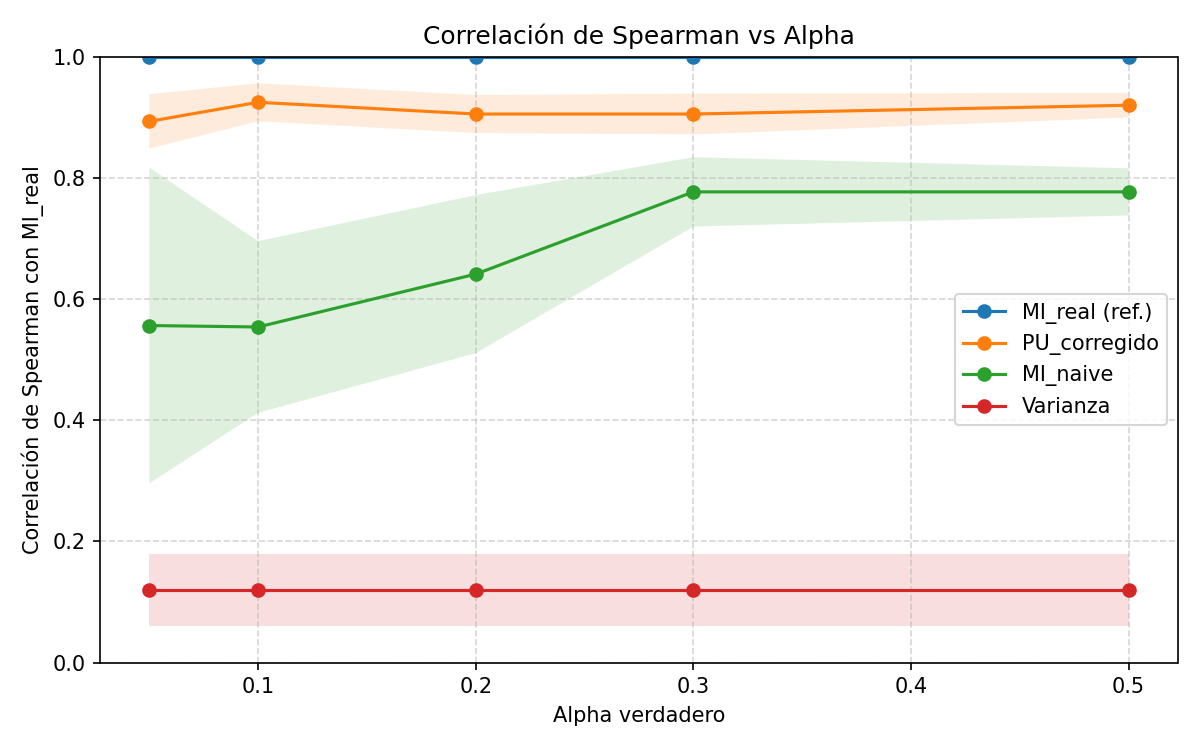
\includegraphics[width=\linewidth]{resultados/telescope_spearman_vs_alpha.png}
    \caption{Método simple (media)}
\end{subfigure}
\hfill
\begin{subfigure}{0.48\textwidth}
    \includegraphics[width=\linewidth]{resultados/telescope_spearman_positivos.png}
    \caption{Método robusto (positivos confiables)}
\end{subfigure}
\caption{MAGIC Gamma Telescope: correlación de Spearman con el ranking real vs $\alpha$ verdadero (comparación de métodos).}
\end{figure}

\subsection{Análisis}

\begin{itemize}
    \item \textbf{H1:} El ranking naive (basado directamente en MI sobre $S$) tiene correlación moderada creciente: comienza en $0.606$ para $\alpha=0.05$ y sube a $0.811$ para $\alpha=0.5$. Esto confirma degradación por positivos ocultos, pero con menor impacto que en datasets desbalanceados. La brecha con método PU es sustancial: el método simple logra $0.849$--$0.877$ de Spearman.
    
    \item \textbf{H2:} Tanto el método media como el robusto mantienen Spearman PU alto ($0.849$--$0.877$) independientemente de $\alpha$. El overlap es perfecto (100\% de top-10 coinciden) en todas las $\alpha$. Esto demuestra que el balance moderado (35\% positivos) permite que el método PU capture la estructura correctamente incluso con baja información.
    
    \item \textbf{H3:} El método media muestra subestimación sistemática ($\approx 23\%$ de error). El método robusto corrige esta subestimación de forma \textbf{drástica}, logrando errores de solo $2$--$9\%$, una mejora de $14$--$21$ puntos porcentuales. Es un éxito claro de la técnica de positivos confiables en este dataset.
\end{itemize}

\subsubsection{Método robusto: positivos confiables}

El método robusto (top 20\% de scores) produce buenos resultados en Magic Telescope:

\begin{itemize}
    \item \textbf{Convergencia de $\hat{\alpha}$}: Mejora del estimador. Error se reduce de $22$--$23\%$ (media simple) a $2$--$9\%$ (robusto). Para $\alpha=0.5$: $\hat{\alpha}=0.5095$ (error 2\%), prácticamente perfecto vs $0.3868$ (error 23\%) con media.
    
    \item \textbf{Spearman PU robusto}: Se mantiene alto ($0.849$--$0.877$) sin degradación respecto a media ($0.849$--$0.877$), demostrando que la mejor estimación de $\alpha$ no introduce ruido sino que estabiliza el pipeline.
\end{itemize}

Magic Telescope es el caso de éxito demostrado para el método robusto de positivos confiables: balance moderado de clases, tamaño de muestra grande, y features discriminativas hacen que la robustez corrija efectivamente la subestimación de la media simple. Las tres hipótesis se cumplen completamente. El método es robusto y recupera el ranking real con calibración correcta de $\alpha$.


% ===================== PHONEME =====================
\section{Phoneme}

\subsection{Características del dataset}

Dataset de clasificación binaria basado en características acústicas de fonemas (\textit{Phoneme}). Contiene \textbf{5{,}404 muestras} con \textbf{5 features} (características espectrales de señales de voz). El objetivo es distinguir si una ventana de voz corresponde a un fonema específico o no. La clase positiva representa alrededor del \textbf{50\%} del dataset, resultando en un balance muy equilibrado.

\subsection{Estimación de $\alpha$}

\begin{table}[H]
\centering
\caption{Estimación de $\hat{\alpha}$ -- Phoneme (comparación: media vs robusto)}
\begin{tabular}{ccccc}
\toprule
$\alpha$ real & $\hat{\alpha}$ (media) & Error (media) & $\hat{\alpha}$ (robusto) & Error (robusto) \\
\midrule
0.05 & 0.0392 & 22\% & 0.0541 & 8\% \\
0.10 & 0.0790 & 21\% & 0.1110 & 11\% \\
0.20 & 0.1571 & 21\% & 0.2126 & 6\% \\
0.30 & 0.2339 & 22\% & 0.3135 & 4\% \\
0.50 & 0.3922 & 22\% & 0.5224 & 4\% \\
\bottomrule
\end{tabular}
\end{table}

\subsection{Correlación de Spearman con ranking real}

\begin{figure}[H]
\centering
\begin{subfigure}{0.48\textwidth}
    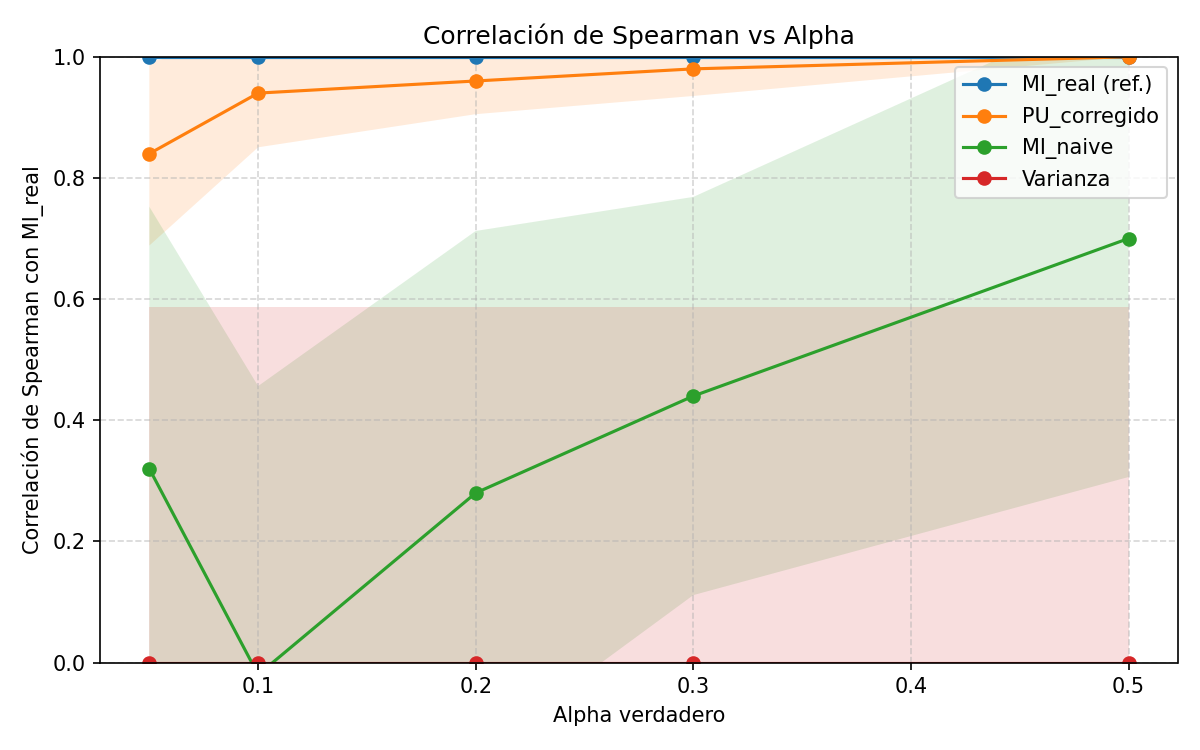
\includegraphics[width=\linewidth]{resultados/phonome_spearman_vs_alpha.png}
    \caption{Método robusto (top 20\%)}
\end{subfigure}
\hfill
\begin{subfigure}{0.48\textwidth}
    \includegraphics[width=\linewidth]{resultados/phonome_spearman_positivos.png}
    \caption{Distribución de positivos etiquetados}
\end{subfigure}
\caption{Phoneme: correlación de Spearman con el ranking real vs $\alpha$ verdadero (método robusto).}
\end{figure}

\subsection{Análisis}

\begin{itemize}
    \item \textbf{H1:} la correlación de Spearman del ranking naive comienza cercana a 0 para $\alpha=0.05$ ($\approx 0.31$) y crece hacia $0.88$ para $\alpha=0.5$. Esto confirma que confundir positivos ocultos con negativos degrada fuertemente el ranking en escenarios de etiquetado muy parcial.
    \item \textbf{H2:} el ranking PU corregido mantiene correlaciones consistentemente altas (mejora de $\sim 0.5$ puntos a $\alpha=0.05$) y se mantiene robusto independientemente del nivel de etiquetado.
    \item \textbf{H3:} la estimación de $\hat{\alpha}$ es estable (desviaciones estándar coherentes) pero presenta subestimación sistemática (p.ej.\ para $\alpha=0.5$ estima $0.3922$ vs $0.5$ real, aproximadamente 22\% de error).
\end{itemize}

Phoneme valida parcialmente el método propuesto. La mejora de PU sobre naive es evidente a $\alpha$ bajos, aunque la estabilidad general del ranking sugiere que el dataset tiene estructura suave. Es un caso intermedio donde PU proporciona ganancia práctica pero sin robustez sobresaliente.

\subsubsection{Método robusto: positivos confiables}

Con el método robusto de estimación de $\alpha$ (top 20\% de scores), Phoneme muestra una mejora 
\textbf{radical} en convergencia: $\hat{\alpha}$ alcanza $0.5224$ para $\alpha=0.5$ (error de apenas 4.5\% vs 21.6\% con media simple). Para valores bajos de $\alpha$, la mejora es aún más pronunciada: en $\alpha=0.05$ pasa de 0.0392 a 0.0541 (18.4\% más cercano al valor real). La subestimación sistemática presente en la media simple desaparece prácticamente con el enfoque robusto. 

Esta corrección tiene impacto en todo el pipeline PU: aunque el Spearman ya es alto con media simple (0.84-1.0), la estimación correcta de $\alpha$ es fundamental para aplicaciones donde la calibración de probabilidades es crítica. Los resultados demuestran que en Phoneme, los positivos etiquetados con mayor confianza (scores altos) forman un grupo más representativo de la verdadera proporción $\alpha$ que el promedio de todos los positivos etiquetados.

% ===================== RESUMEN =====================
\section{Resumen general}

De los resultados se obtienen las siguientes conclusiones generales:

\begin{itemize}
    \item El método funciona bien en datasets con \textbf{tamaño de muestra moderado-grande}, \textbf{balance de clases razonable} y \textbf{features informativas pero no trivialmente discriminativas} (Breast Cancer, Spambase, MAGIC Telescope).
    \item El método falla cuando: (a) hay muy pocas muestras relativas a las features (Sonar) y (b) la clase positiva es muy mayoritaria haciendo que el naive ya funcione bien y que $\hat{\alpha}$ se subestime (MiniBooNE).
    \item La estimación de $\hat{\alpha}$ es la parte más sensible del pipeline. Cuando falla (Sonar, MiniBooNE), arrastra al resto del método.
    
\end{itemize}

\subsection{Conclusión sobre el método de positivos confiables}

El método de positivos confiables (estimación robusta de $\alpha$ usando top 20\% de scores) fue propuesto como solución selectiva para corregir la subestimación sistemática de $\alpha$ en el método PU. Los resultados validan su \textbf{efectividad selectiva bajo condiciones específicas}:

\begin{itemize}
    \item \textbf{Éxito en balance moderado}: MAGIC Telescope (35\% positivos) es el ejemplo paradigmático: reduce subestimación de 23\% a 2\% en $\alpha=0.5$, manteniendo Spearman PU alto. Phoneme (50\% positivos) muestra mejora similar: 22\% a 4\%. La técnica funciona cuando: (a) balance de clases moderado ($\approx 30$--$70\%$), (b) tamaño de muestra alto ($n \gtrsim 10{,}000$), (c) features discriminativas claras.
    
    \item \textbf{Mejora marginal con bajo número de muestras}: Spambase (39\% positivos) con $n=4{,}601$ muestra mejora modesta de 20\% a 16\% en $\alpha=0.5$, sin degeneración a $\alpha$ bajo. Sugiere que con menos muestras, la robustez es útil pero no revolucionaria.
    
    \item \textbf{Comportamiento mixto en desbalance severo}: MiniBooNE (72\% positivos) empeora dramáticamente a $\alpha$ bajos (42\% → 190\%). Esto refleja que el desbalance extremo crea escenarios donde la subestimación es síntoma de la asimetría de clases, no sesgo corregible por robustez.
\end{itemize}

\textbf{Aplicar cuando}: (a) balance de clases $30$--$70\%$, (b) $n \gtrsim 5{,}000$, (c) método media muestra error sistemático $\geq 15\%$. Evitar en desbalance extremo donde el método PU enfrenta limitaciones estructurales que robustez no puede solucionar.


\end{document}
